\documentclass[aps,twocolumn,secnumarabic,balancelastpage,amsmath,amssymb,nofootinbib,floatfix]{revtex4-1}

\usepackage[colorlinks=true,linkcolor=blue]{hyperref} 

\usepackage{mathexam}
\usepackage{booktabs}

%\usepackage{a4wide}
\usepackage[utf8]{inputenc}
\usepackage{amsmath}
\usepackage{amsfonts}
\usepackage{amssymb}
\usepackage{mathtools}
\usepackage[brazil]{babel}
%quebra de linha do sumário
%\usepackage[breaklinks=true]{hyperref}
%\usepackage{braket}
\usepackage{minitoc}
\usepackage{wrapfig}
\usepackage{subfigure}
\usepackage{setspace}
\usepackage{indentfirst}


\usepackage{physics}


\newtheorem{definition}{Definição}

\usepackage{accents}


\usepackage{blindtext}

\usepackage{graphicx}

%\onehalfspacing


\newcommand*{\dt}[1]{%
  \accentset{\mbox{\large\bfseries .}}{#1}}
\newcommand*{\ddt}[1]{%
  \accentset{\mbox{\large\bfseries .\hspace{-0.25ex}.}}{#1}}
\newcommand*{\dddt}[1]{%
  \accentset{\mbox{\large\bfseries .\hspace{-0.25ex}.\hspace{-.20ex}}}{#1}}
\newcommand*{\dnt}[2][4]{\dt{#2}^{\tiny(#1)}}

\newcommand{\esimo}{-\text{ésimo}}
\newcommand{\esima}{-\text{ésima}}

\makeatletter
\newcommand*{\gnuplotinput}[2][1.0]{%
  \begingroup
  \let\@gnplt@input@includegraphics=\includegraphics
  \def\includegraphics##1{\@gnplt@input@includegraphics[scale=#1]{#2}}%
  \let\@gnplt@input@picture=\picture
  \def\picture{\unitlength=#1\unitlength\relax\@gnplt@input@picture}%
  \input{#2}%
  \endgroup
}
\makeatother


\makeatletter
\newcommand*{\customclear}{%
  \close@column@grid
  \cleardoublepage
  \twocolumngrid
}
\makeatother


\newcommand{\paragr}[1]{\textbf{#1\ }}


\usepackage{listings}
\usepackage{color}

\definecolor{mygreen}{rgb}{0,0.6,0}
\definecolor{mygray}{rgb}{0.85,0.85,0.85}
\definecolor{mymauve}{rgb}{1,0.502,0}
\definecolor{numGray}{rgb}{0.3,0.3,0.3}


\lstdefinestyle{CStyle}{language=C,	
  backgroundcolor=\color{mygray},   % choose the background color; you must add \usepackage{color} or \usepackage{xcolor}; should come as last argument
  basicstyle=\footnotesize,        % the size of the fonts that are used for the code
  breakatwhitespace=false,         % sets if automatic breaks should only happen at whitespace
  breaklines=true,                 % sets automatic line breaking
  captionpos=b,                    % sets the caption-position to bottom
  commentstyle=\color{mygreen},    % comment style
  deletekeywords={...},            % if you want to delete keywords from the given language
  escapeinside={\%*}{*)},          % if you want to add LaTeX within your code
  extendedchars=true,              % lets you use non-ASCII characters; for 8-bits encodings only, does not work with UTF-8
  frame=single,	                   % adds a frame around the code
  keepspaces=true,                 % keeps spaces in text, useful for keeping indentation of code (possibly needs columns=flexible)
  keywordstyle=\color{blue},       % keyword style
  language=C,                 % the language of the code
  morekeywords={*,...},            % if you want to add more keywords to the set
  numbers=left,                    % where to put the line-numbers; possible values are (none, left, right)
  numbersep=5pt,                   % how far the line-numbers are from the code
  numberstyle=\tiny\color{numGray}, % the style that is used for the line-numbers
  rulecolor=\color{black},         % if not set, the frame-color may be changed on line-breaks within not-black text (e.g. comments (green here))
  showspaces=false,                % show spaces everywhere adding particular underscores; it overrides 'showstringspaces'
  showstringspaces=false,          % underline spaces within strings only
  showtabs=false,                  % show tabs within strings adding particular underscores
  stepnumber=1,                    % the step between two line-numbers. If it's 1, each line will be numbered
  stringstyle=\color{mymauve},     % string literal style
  tabsize=2,	                   % sets default tabsize to 2 spaces
  title=\lstname                   % show the filename of files included with \lstinputlisting; also try caption instead of title
}


\newtheorem{theorem}{Teorema}

\newcommand{\conf}[1]{ \{ #1 \} }
\newcommand{\sconf}{\conf{\sigma}}
\newcommand{\sz}{\hat{\sigma}^z}
\newcommand{\sx}{\hat{\sigma}^x}
\newcommand{\sy}{\hat{\sigma}^y}
\newcommand{\aOper}{\hat{a}}
\newcommand{\aDagg}{\aOper^\dagger}
\newcommand{\cOpr}{\hat{c}}
\newcommand{\cDagg}{\cOper^\dagger}
\newcommand{\bq}{\beta_q}
\newcommand{\bcl}{\beta_{cl}}
\newcommand{\ham}{\hat{H}}
\newcommand{\oper}{\mathcal{O}}

\usepackage{tensor}
\begin{document}
\title{Mapeamento Clássico-Quântico - Estudando o Emaranhamento Quântico  simulando Modelos Clássicos para o Modelo de Ising}
\author{Alex Enrique Crispim}
%\affiliation{Estudante de graduação - Bacharelado em Física, Universidade Federal do ABC}
\email{alex.enrique@aluno.ufabc.edu.br}

\begin{abstract}
Neste trabalho exploraremos a técnica do mapeamento clássico-quântico, com base no Modelo de Ising. De forma geral, acredita-se que a função de partição de um modelo quântico de dimensão $D$ possa ser mapeada na função de partição de uma modelo clássico de dimensão $D+1$. Aplicando-se tal técnica ao Modelo de Ising Quântico, podemos calcular observáveis quânticos por meio de simulações computacionais do Modelo Clássico. Por meio do método de Monte Carlo, jutamente com o Algoritmo de Metropolis, calcularemos observáveis quânticos e veremos a vantagem de tal procedimento. Esta abordagem nos permitirá estudar propriedades de emaranhamento a respeito do sistema quântico por meio do sistema clássico. Ao final, seremos levados à hipótese de que a transição de fase no Modelo de Ising se mostra como uma transição de fase da forma localidade$-$não localidade, onde as desigualdades de Bell passam a ser violadas.
\end{abstract}

\maketitle

\tableofcontents

\section{Introdução}
\label{sec:Introducao}

\subsection{Contextualização} 
\label{subsec:Contextualizacao}

O Modelo de Ising surgiu no início da década de 1920. O mesmo foi cunhado por Wilhelm Lenz, o qual delegou o trabalho sobre o modelo ao seu orientando Ernest Ising. O modelo original era um \textit{modelo clássico} no sentido que as variáveis (spins) comutavam; eram representadas por números como $+1$ e $-1$. \cite{IsingIntro}

De início, o modelo visava estudar e entender os fenômenos de ferromagnetismo e transição de fase ferromagnética-paramagnética. Ainda que sem sucesso de início, com o resultado de que não haveria transição de fase para o modelo em uma dimensão, resultado apresentado por Ising que o levou a concluir que o modelo não apresentaria uma transição de fase para nenhuma dimensão \cite{Ising}, em  1936 R. Peirls mostrou o surgimento de transições de fase para dimensões maiores do que dois \cite{Peierls-1936}. 

Posteriormente, já no início da década de 1940, é publicada a chamada \textit{dualidade de Krammers-Wannier} para o Modelo de Ising  \cite{Kramers-1941I, Kramers-1941II}. Tal dualidade se apresenta como uma relação de simetria intrinseca do modelo. A utilização da mesma posibilitou aos autores estabelescer a temperatura de transição de fase para o modelo, sob a hipótese de que a mesma deveria ser única. A apresentação dos supracitados resultados foram apresentada em uma conferência onde \textit{Lars Onsager} se encontrava presente. Ao final, Onsager anunciar ter encontrado a solução exata para o modelo bi-dimensional e que o resultado obtido era o mesmo apresentado por Krammers e Wannier \cite{FiftyYears}. Em 1944, Onsager publica a solução exata para o modelo, na ausencia de campo magnético externo \cite{Onsager1944}. 

A solução encontrada, no entanto, não permitia a avaliação direta da magnetização resultante após a remoção de um campo magnético externo não nulo. Entretanto, em 1949, Onsager determina uma dependência entre a magnetização resultante e a razão $T/T_c$, onde $T$ representa a temperatura e $T_c$ a temperatura de transição de fase para o modelo. A publicação só se deu em 1952 por Yang \cite{Yang}. 

Tinha-se então o primeito modelo a apresentar uma transição de fase, históricamente \cite{FiftyYears}. Foi o marco do início do estudo de transições de fase, futuramente levando a avanços significativos para a Física de muitos corpos.


Tempos depois, mostrou-se que a Hamiltoniana de Ising (clássica) pode ser mapeada numa Hamiltoniana quântica, se se considera uma das dimensões do modelo como sendo uma dimensão espacial \cite{KogutMain, FradSussk}. Tal procedimento introduz uma anisotropia na rede \cite{KogutMain, FradSussk}. O Modelo de Ising passa a ser a base para o entendimento de transições quânticas de fase e a construção do mapeamento clássico-quântico se torna fundamental para o entendimento de teorias fortemente correlacionadas. 

\subsection{Objetivo}
\label{subsec:Objetivo}
O objetivo deste trabalho é apresentar brevemente o mapeamento de um problema quântico de Ising em um problema clássico de forma a simular os valores esperados quânticos utilizando-se do problema clássico, com algoritmos menos custosos computacionalmente \cite{IsingSim}. Apresentar as vantagens e desvantagens de tal construção teórica e apresentar o Método de Monte Carlo e o Algoritmo de Metrópolis para o cálculo de observáveis em mecânica estatística clássica. 

\section{Teoria e Metodologia}
\label{sec:TeoriaEMetodologia}
Esta seção busca desenvolver, de forma simples, os conhecimentos necessários para se entender a física em questão e apresentar a métodologia do trabalho; como os observáveis foram calculados. 

\subsection{O Modelo Clássico e o Modelo Quântico de Ising}
\label{subsec:OModeloClassicoeoModeloQuantico}

O Modelo de Ising é o modelo de vértices mais simples que se pode construir (tanto quântico como clássico), seguido do modelo de Heisenberg. Trataremos do modelo numa rede quadrada.

De forma geral, modelo clássico consiste em um hipercubo $\Omega$ em um espaço de dimensão $d$, $\mathbb{Z}^d$,
\begin{equation*}
	\Omega = [-a, a] \times ... \times [-a, a] \cap \mathbb{Z}^d \qc a > 0,
\end{equation*}
com o produto cartesiano sendo tomado $d$ vezes. $\Omega$ é uma estrutura a qual é chamama \textit{rede}. Cada elemento da rede é denominado \textit{sítio}, sendo cada sítio descrito por uma $d-$upla; por exemplo $i = (i_1, ..., i_d)$. 

Para cada sítio, existe uma associação bijetiva que mapeia-o em uma variável $\sigma$, denominada \textit{spin};
\begin{equation*}
	\Omega \to \mathcal{D}_\Omega; \ \ i \mapsto \sigma_i.
\end{equation*}
A variável spin é tomada como pertencendo a um \textit{grupo abeliano}. Isso significa que existe uma operação $"\cdot"$ denotada \textit{produto} definida entre dois spins, de sítios diferentes, tal que a operação é comutativa. O fato de ser comutativa difere o modelo clássico do modelo quântico, a ser apresentado ainda nesta subseção.

Usualmente, o grupo a qual os spins pertencem são números reais, no máximo. Para muitos casos, também o deste trabalho, tomaremos que os spins podem assumir os valores do conjunto $\{-1, +1\}$. Formalmente,

\begin{definition}
	Dada uma rede $\Omega$ com spins $\sigma_i$ associados a cada sítio $i$. Então, chama-se uma \textit{configuração de spins}, denotada $\{ \sigma \}$, o mapa 
	\begin{flalign*}
		\{ \sigma \} : \Omega &\to \{ -1, 1\}^{\abs{\Omega}} \\
		i & \mapsto \sigma_i 
	\end{flalign*}
\end{definition}

A Figura \ref{fig:II.1} ilustra uma rede para $d = 2$ e de cardinalidade $16$. 

\begin{figure}[h]
	\center
	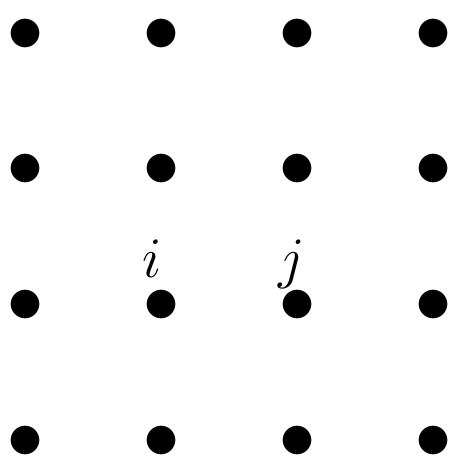
\includegraphics[scale=.2]{rede2d.png}
	\caption{Rede quadrada (d=2)}
	\label{fig:II.1}
\end{figure}

Ernerst Ising, em seu trabalho, formulou duas premissas \cite{Ising}. As premissas apresentadas se justificam por uma crítica à \textit{hipótese do campo molecular}, para o ferromagnetismo, devida a Weiss. Ising toma como premissa que a interação entre os spins da rede deve decair muito rapidamente, de tal forma que podemos tomar o que se chama de primeiros vizinho \cite{Ising}. Definiremos mais formalmente logo abaixo.

A segunda premissa é a de que os elementos constintuintes do sistema ocupam apenas alguns níveis distintos de energia e que a energia interna é a mínima para quando os spins estão alinhados (para o caso do ferromagnetismo). Excitações térmicas devidas a um acoplamento com um banho seriam responsáveis pela população de outros níveis de energia. \cite{Ising}

Mais formalmente,
\begin{definition}
	Seja $\norm{\cdot}$ a métrica definida como 
	\begin{flalign*}
		\norm{\cdot} \colon \mathbb{Z}^d &\to \mathbb{Z} \\
		 i &\mapsto \max\{\abs{i_k}\qc k = 1,..., d\}
	\end{flalign*}
	
	Chamamos os $j$ primeiros vizinhos de $i$, denotado $\ev{i, j}$, o conjunto
	\begin{equation*}
		\ev{i, j} = \{j \in \mathbb{Z}^d \colon \norm{j - i} = 1 \}
	\end{equation*}
\end{definition}

Seja $V_{ij}$ a interação entre dois spins $\sigma_i$, $\sigma_j$, as hipóteses para o modelo levam a
\begin{equation*}
	V_{ij} \propto \sigma_i \sigma_j = J_{ij} \sigma_i \sigma_j; \quad J_{ij} \sim \norm{i-j}^{-\alpha}, \alpha > 0. 
\end{equation*}
O termo $J_{ij}$ é chamado \textit{termo de troca} ou \textit{acoplamento} entre os spins $i$ e $j$\footnote{Por vezes, nos referimos aos spins mencionando suas localizações, visto que o mapa $\{ \sigma \}$ é bijetivo.}
A energia da rede, para uma dada configuração $\{ \sigma \}$ se dá pela energia de interação entre os spins e a possível interação dos mesmos com algum agente externo. Para o caso do ferromagnetismo, a interação com agentes externos é justamente a interação com o campo magnético externo. 

Matemáticamente, a energia é
\begin{equation}
	H( \{ \sigma \} ) = - \sum_{\ev{i,j}} J_{ij} \sigma_i \sigma_j - \sum_i B_i \sigma_i,
	\label{eq:II.1}
\end{equation}
onde $J_{ij}$ é o termo de troca e $B_i$ é o coeficiente que descreve a interação do spin $i$ com o campo magnético externo. O simbolo $\ev{i,j}$ presente na primeira soma significa que a soma é feita sobre os $j$ primeiros vizinhos de $i$, para cada $i$ em $\Omega$. 

A equação (\ref{eq:II.1}) é chamada \textit{Hamiltoniana de Ising}, para o modelo clássico. 

Costumeiramente, toma-se os acoplamentos $J_{ij}$ iguais, ao menos para cada indíce fixo de $i$ e $j$, ou seja, para o índice $i_k$ de $i$, todas as constantes são iguais, para cada $k$. 

Abaixo apresentamos dois exemplos. 
\begin{flalign}
	H(\{ \sigma \}) &= -J \sum_i \sigma_i \sigma_{i+1} - B \sum_i \sigma_i, \label{eq:II.2} \\
	H(\{ \sigma \}) &= -J_1 \sum_{i,j} \sigma_i^j \sigma_{i+1}^j - J_2 \sum_{i,j} \sigma_i^j \sigma_i^{j+1}. \label{eq:II.3}
\end{flalign}

A hamiltoniana (\ref{eq:II.2}) representa o modelo em uma dimensão, com acoplamento igual para todos os spins e mesma ação devido ao campo magnético e (\ref{eq:II.3}) represente um modelo de hamiltoniana em duas dimensões, denotadas pelos indices subscritos e sobrescritos em $\sigma$, com acoplamento anisotrópico na direção vertical e horizontal ($J_1$ e $J_2$) e na ausência de campo magnético. 

O trabalho de Ising constitiu na análise da hamiltoniana (\ref{eq:II.2}), concluindo que não haveria trasição de fase para uma dimensão. Com alguns argumentos, Ising afirma que não haveria para qualquer dimensão. Sua tese fora publicada dessa forma. Até que, futuramente, se mostrou haver uma transição de fase para o dimensões maiores ou iguas a 2. O trabalho de Onsager produziu uma solução exata para a hamiltoniana em (\ref{eq:II.3}).

Com um pouco de análise, pode-se mapear a hamiltoniana em (\ref{eq:II.3}) numa hamiltoniana quântica dada por \cite{KogutMain, FradSussk}
\begin{equation}
	\ham = -J \sum_{i} \sz_i \sz_{i+1} + \lambda \sx_i .  
	\label{eq:II.4}
\end{equation}

Os operadores $\sz$ e $\sx$ são os operadores de spin dados pelas matrizes $Z$ e $X$ de Pauli \cite{QuantumCompInf}. A hamiltoniana em (\ref{eq:II.4}) representa a tendência dos spins de alinharem na direção $\sz$ e um campo transverso $\sx$, mediado pelo termo $\lambda$. O parâmetro $\lambda$ equivale à temperatura do modelo clássico\footnote{Não proporcionalmente.}. À temperatura zero, os spins tendem a se alinhar em $\sz$ para minimizar a energia, estando em um dos estados chamados \textit{estado de Néel}. Quando se tem a temperatura, ocorre a ação do termo $\sx$ que, ao se medir na auto-base do operador $\sz$ faz surgir os \textit{flips}. 

A passagem de (\ref{eq:II.3}) para (\ref{eq:II.4}) não é feita de forma trivial. Um dos passos mais importantes é tomar uma das dimensões da hamiltoniana clássica como sendo uma dimensão espacial imaginária, mapeando-se um espaço euclidiano de dimensão (2+0) em um espaço de Minkowski de dimensão (1+1). Para maiores detalhes: \cite{KogutMain, FradSussk}. 

Em vista do mapeamento de (\ref{eq:II.3}) em (\ref{eq:II.4}), podemos calcular observáveis em cada um dos dois modelos e determinar equivalentes no outro. Neste trabalho, utilizou-se a técnica do mapeamento clássico-quântico para o cálculo de observáveis quânticos por meio de simulações do sistema clássico. 

A partir desta subseção, a base para o entendimento do que será estudado sobre o modelo de Ising, neste trabalho, está fundamentada. Conceitos importantes de termodinâmica e mecânica estatística foram deixados para a subseção \ref{subsec:VariaveisTermodinamicasEMecanicaEstatistica}.

\subsection{Variáveis Termodinâmicas e Mecânica Estatística}
\label{subsec:VariaveisTermodinamicasEMecanicaEstatistica}

O fenômeno de ferromagnetismo; o alinhamento preferêncial dos spins do material, é estudado via Modelo de Ising por meio de dois princípios fundamentais que governam a dinâmica dos spins: \textit{minimização de energia} e \textit{maximização da entropia}. O entendimento destes dois últimos conceitos se dá no âmbito da termodinâmica e da mecânica estatística.

Um sistema termodinâmico é completamente determinado por uma função $f(p, V, T, ...)$ chamada \textit{função de estado}, onde as variáveis que recebe são as que descrevem todo o sistema termodinamicamente \cite{Schroeder}. Existem funções de estado específicas denominadas \textit{potenciais termodinâmicos} das quais algumas recebem o nome de \textit{função energia livre}. As mais comuns funções são as energia livre de Gibbs, de Helmholtz e a Entalpia \cite{Huang, Schroeder}.

A energia livre de Helmholtz $F = U - TS$, com $U$ sendo a energia interna, $T$ a temperatura e $S$ a entropia do sistema, tem a seguinte forma diferencial
\begin{equation}
	\dd{F} = \dd{U} - T \dd{S}.
	\label{eq:II.5}
\end{equation}

A entidade em (\ref{eq:II.5}) é o que descreve a ideia de minimizar a energia e maximizar a entropia. Note que uma redução em $U$, acarreta em uma redução em $F$. Em contraposição, um aumento em $S$, leva a uma redução de $F$ \cite{Schroeder}. 

Para o Modelo de Ising clássico, o estado fundamental é composto por todos os spins apontando em uma direção. Considere o modelo unidimensional para melhor entendimento. Se um spin é flipado na posição $i$ e outro na posição $j$ da rede, há um aumento de energia, se a configuração anterior corresponderia ao estado fundamental. Considerando agora que se o spin $j$ seja $i+2$, fazendo um \textit{flip} na posição $i+1$, pode-se ver que a energia do sistema é a mesma que se $j$ fosse o sítio $i+3$ e os spins $i+1$ e $i+2$ estivessem sofrido um \textit{flip}. Da mesma forma, escolhidas duas posições $i$ e $j$ quaisquer distintas, a energia do sistema para o qual todos os spins entre as posições escolhidas também sofreram um flip é a mesma que das configurações  anteriores.

O último exemplo  ilustra como estados de mais alta energia apresentam mais configurações possíveis para a mesma energia; uma espécie de degenerescência. Esse maior número de configurações significa uma maior entropia. Vê-se, portanto, que um aumento na entropia está fortemente relacionado a um aumento na energia. A equação (\ref{eq:II.5}) representa uma "disputa" $ $ entre energia e entropia. Essa dinâmica é justamente a dinâmica do sistema dado pelo Modelo de Ising \cite{Huang, Baxter}. 

\vspace*{1.5mm}
\paragr{Distribuição de Boltzmann -} Partindo da energia livre, podemos chegar ao chamado \textit{peso de Boltzmann}, o qual é responsável pela distribuição de Boltzmann. O peso de Boltzmann é dado por
\begin{equation}
	P (\sconf) = e^{-\beta H(\sconf)}, 
	\label{eq:II.6}
\end{equation}
onde $\beta = 1/kT$, com $k$ representando a \textit{constante de Boltzmann}. A normalização do peso de Boltzmann leva a medida de probabilidade 
\begin{equation}
	\mu_\beta (\sconf) = \frac{1}{Z} e^{-\beta H(\sconf)} \qc Z = \sum_{\sconf} e^{-\beta H(\sconf)}.
	\label{eq:II.7}
\end{equation}

$Z$ é uma entidade chamada \textit{função de partição}. A soma é feita sobre todas as configurações de spin $\sconf$. A distribuição de probabilidade (\ref{eq:II.7}) descreve a dinâmica dos Modelos Clássicos e Quânticos de Ising, uma vez que ambos funcionam sobre os mesmos princípios de minimização da energia livre. As últimas expressões serão utilizadas na criação do algoritmo para a simulação da dinâmica da rede de spins.

Uma vez dada a energia de cada estado possível, a medida (\ref{eq:II.7}) fornece a probabilidade de cada estado (para uma dada temperatura) \cite{Huang, Schroeder}. Quantidades macroscópicas podem então ser calculadas fazendo uso da distribuição de probabilidade do sistema. A energia média por exemplo pode ser obtida como\footnote{Passaremos a fazer uso da convenção de que quando a configuração de spins for argumento de uma função, omitiremos as chaves $\{ \ \}$.}
\begin{equation}
	\ev{H} = \sum_{\sconf} H(\sigma) \mu_\beta(\sigma) = \frac{1}{Z} \sum_{\sconf} H(\sigma) e^{-\beta H(\sigma)}.
	\label{eq:II.8}
\end{equation} 

Expressões como (\ref{eq:II.8}) são inviáveis de se calcular configuração a configuração, visto que o espaço de configurações de spins $\sconf$ cresce com cardinalidade $2^N$, onde $N$ é o número de spins. Se faz necessário um método  para o cálculo de observáveis médios utilizando um algoritmo computacionalmente menos custoso.  \cite{IsingSim}



\subsection{Amostrando-se o Espaço de Fase e Calculando-se Médias}
\label{subsec:AmostrandoseECalculandoseMedias}

Um meio de se calcular observáveis médios como em (\ref{eq:II.8}) é amostrando o espaço de fase do sistema de forma a tomar as regiões de maior probabilidade de ocorrência com maior frequência que regiões de baixa probabilidade. Para tal, utilizamos a distribuição de probabilidade do próprio sistema estatístico. 

Seja $x$ um ponto do espaço de fase, o valor médio de um observável para a temperatura $T$ em um ensamble canônico é
\begin{equation*}
	\ev{A(x)}_T = \frac{1}{Z} \int \dd{x} A(x) e^{-\beta H(x)},
\end{equation*}
ou, para um caso discreto, 
\begin{equation*}
	\ev{A(x)}_T = \frac{1}{Z} \sum_{x} A(x) e^{-\beta H(x)}. 
\end{equation*}

Consideramos uma porção finita do espaço de fase. Precisamos garantir que a distribuição estará com pico na região a ser considerada. Fazemos uso agora da ideia de se escolher os pontos do espaço de fase de acordo com a disribuição própria do sistema. Escolhendo os pontos $x$ do espaço de fase desta forma, o valor médio para $A$ passa a ser
\begin{equation*}
	\ev{A} = \frac{\sum_{l=1}^M e^{-\beta H(x_l)} A(x_l)/p(x_l)}{\sum_{l=1}^M e^{-\beta H(x_l)}/p(x_l)} = \frac{1}{M} \sum_{l=1}^N A(x_l). 
\end{equation*}

A equação acima é uma tentativa de se reduzir a distribuição de probabilidade de um espaço de fase infinito, (correpondente ao limite onde o número de spins tende para infinito) por meio de uma porção da rede, com um número finito $M$ de pontos $x_l$ \cite{IsingSim}. A abordagem acima é um modo mais simples de se tratar o \textit{Teorema Ergódico}. Apresentaremos o resultado de forma mais formal após tratarmos de cadeias de Markov em \ref{subsec:MonteCarloEMetropolis}.

A geração do conjunto $\{x_l\}$ é feita pelo \textit{algoritmo de Metropolis}. Utilizamos, com isso, o método de Monte Carlo para o cálculo do valor médio de um observável $A$.


\subsection{Monte Carlo e o algoritmo de Metropolis}
\label{subsec:MonteCarloEMetropolis}

O Método de Monte Carlo consiste em realizar cálculos por meio de amostragem estatística, fazendo uso de distribuições de probabilidades ou para o cálculo de probabilidades. O método consiste em sortear, um grande número de vezes, estados possíveis para uma quantidade a qual queremos calcular e então determinar a mesma de forma estatística. 

Para o cálculo do valor médio de um observável, o sorteio supracitado se refere a sortear valores possíveis deste observável. A geração do conjunto de valores é então feita pelo já citado algoritmo de Metropolis. 

O algoritmo de Metropolis faz uso das \textit{cadeias de Markov}. 

\vspace*{1.5mm} 
\paragr{Cadeias de Markov - } Considere uma sequência de variáveis aleatórias $\Gamma=( \Gamma_1, \Gamma_2, ... )$ onde as variáveis $\Gamma_i$ tomam valores no conjunto das possíveis configurações de spin $\sconf$ da rede. Neste sentido, $\Gamma_k$ representa a configuração do sistema no instante $k$. Se para cada instante $k$ e configuração $\Gamma_k = \conf{\sigma_k}$ que o sistema pode assumir existir uma probabilidade $p_{kj}$ de o sistema passar da configuração $\conf{\sigma_k}$ para a configuração $\conf{\sigma_j}$, então a sequência $\Gamma$ chama-se cadeia de Markov. $p_{kj}$ chamam-se \textit{probabilidade de transição}.

Note que o fato de para cada instante existir tal probabilidade significa que o passo seguinte independe dos anteriores; a dinâmica da rede é sem memória. 

É fácil ver que este é o caso para o Modelo de Ising. Se em algum instante, o sistema está na configuração $\{\sigma_k\}$, para toda configuração $\{ \sigma_j \}$, com $j \neq k$, existe uma probabilidade de transição entre os estados $j$ e $k$, a depender da distribuição (\ref{eq:II.7}), responsável pela dinâmica de redução da energia livre. 

\vspace*{1.5mm}
\paragr{Cadeias Ergódicas - } Um importante ponto a se notar é que a probabilidade de transição 
\begin{equation*}
	p^{(n)}_{ij} = \mu_\beta (\Gamma_{n+m} = \conf{\sigma_j} \vert \Gamma_m = \conf{\sigma_i})
\end{equation*}
é sempre positiva. A mesma recee o nome de probabilidade de transição entre $n$ estados. Cadeias que tem tal propriedade ($p_{ij}^{(n)} > 0$) são \textit{cadeias ergódicas}. Para entender melhor, precisamos de alguns conceitos de teoria de medidas.

\begin{definition}
	Seja $\mathcal{X}$ um conjunto não vázio e $\mathcal{P}(\mathcal{X})$ o conjunto das partes de $\mathcal{X}$ . O subconjunto $\Sigma \subset \mathcal{P}(\mathcal{X})$ é chamado uma \textbf{$\sigma$-álgebra}  se
	\begin{itemize}
		\item[1.] $\mathcal{X} \in \Sigma$ e $\mathcal{X}$ é o conjunto universo, no dado contexto.
		\item[2.] $\Sigma$ é fechado sob complementação, i.e., se $A \in \Sigma$, então $A \backslash \mathcal{X} \in \Sigma$.
		\item[3.] $\Sigma$ é fechado sob uniões contáveis, i.e., se $A_1, ... A_n\in \Sigma$, então $\bigcup_{i=1}^n A_i \in \Sigma$.
	\end{itemize}
\end{definition}

\begin{definition}
	Seja $\mathcal{X}$ um conjunto e $\Sigma \subset \mathcal{P}(\mathcal{X})$ uma $\sigma$-álgebra. Uma \textbf{medida} $\mu$ é um mapa $\mu \colon \Sigma \to I \subset \mathbb{R}$ satisfazendo
	\begin{itemize}
		\item[1.] Não negtividade: Para todo $A \in \Sigma$, $\mu(A) \geq 0$.
		\item[2.] Medida nula para $\emptyset$ $\mu(\emptyset) = 0$.
		\item[3.] Aditividade contável: $\mu \qty(\bigcup_{i=1}^\infty A_i) = \sum_{i=1}^\infty \mu (A_i)$.
	\end{itemize}
	\label{def:4}
\end{definition}
Em especial $\mu$ (definição \ref{def:4}) recebe o nome de medida de probabilidade quando o contradomínio em questão é $I = [0, 1]$. 

\begin{definition}
	Chama-se um \textbf{espaço mensurável} a dupla ($\mathcal{X}, \Sigma$), onde $\mathcal{X}$ é um conjunto não vázio e $\Sigma$ é uma $\sigma$-álgebra sobre $\mathcal{X}$.
\end{definition}

\begin{definition}
	Chama-se um \textbf{espaço de medida} a tripla ($\mathcal{X}, \Sigma, \mu$), onde $\mathcal{X}$ é um conjunto não vázio, $\Sigma$ é uma $\sigma$-álgebra sobre $\mathcal{X}$ e $\mu$ é uma medida em $(\mathcal{A}, \Sigma)$. 
\end{definition}

\begin{definition}
	Sejam $(\mathcal{X}, \Sigma^1)$ e $(\mathcal{Y}, \Sigma^2)$ espaços mensuáveis, a aplicação $T\colon \mathcal{X} \to \mathcal{Y}$ é dita uma \textbf{transformação mensurável} se
	\begin{equation*}
		T^{-1}(A) = \{x \in \mathcal{X} \vert T(x) \in A \} \in \Sigma\qc \forall A \in \Sigma^2.
	\end{equation*}
	Quando satisfeita a condição acima, às vezes escreve-se $T \colon (\mathcal{X}, \Sigma^1) \to (\mathcal{Y}, \Sigma^2)$.
\end{definition}

\begin{definition}
	A transformação $T \colon (\mathcal{X}, \Sigma) \to (\mathcal{X}, \Sigma)$ é uma \textbf{transformação mensuável que preserva a medida $\mu$} se $\mu(T^{-1}(A)) = \mu(A)$, para todo $A \in \Sigma$. À quadrupla $(\mathcal{X}, \Sigma, \mu, T)$ chamamos \textbf{sistema dinâmico que preserva a medida}. 
\end{definition}

\begin{definition}
	Seja $(\mathcal{X}, \Sigma, \mu, T)$ um sistema dinâmico que preserva medida. Então $T$ é \textbf{ergódica} se, para cada $A \in \Sigma$, com $T^{-1}(A) = A$, ou $\mu(A) = 1$ ou $\mu(A) = 0$. 
\end{definition}

\begin{definition}
	Sejam $(\mathcal{X}, \Sigma)$ um espaço mensurável e $f\colon A \in \Sigma \to \mathbb{R}$. $f$ é dita $\Sigma$-mensuável se 
	\begin{equation*}
		\forall k \in \mathbb{R}, \{ x \in A \colon f(x) \leq k \} \in \Sigma.
	\end{equation*}
	O conjunto de tais funções é denotado $\mathcal{M}(\Sigma)$.
\end{definition}

\begin{definition}
	Um \textbf{espaço $\Sigma$-mensuável positivo extendido de funções reais}, denotado $\mathcal{M}^+_{\bar{\mathbb{R}}}(\Sigma)$, é por definição
	\begin{equation*}
		\mathcal{M}^+_{\bar{\mathbb{R}}}(\Sigma) = \{f \colon \mathcal{X}	 \to \bar{\mathbb{R}} \colon f \text{ é $\Sigma$-mensurável } e f \geq 0\},
	\end{equation*}
	onde $\bar{\mathbb{R}} = \mathbb{R} \cup \{ - \infty, + \infty \}$ é o conjunto dos reais extendidos. 
\end{definition}


\begin{definition}
	Seja $(\mathcal{X}, \Sigma, \mu)$ um espaço mensurável e $f \in \mathcal{M}^+_{\bar{R}}$. $f$ é dita ser $\mu$-integrável se
	\begin{equation*}
		\int f^+ \dd{\mu} < +\infty \quad \text{e} \quad \int f^- \dd{\mu} < +\infty,
	\end{equation*}
	com $f^\pm$ denotando as partes positivas e negativas de $f$, respectivamente. 
\end{definition}


Com as definições acima, podemos dar significado ao nome \textit{transformação ergódica} e enunciar o Teorema Ergódico.


É fácil ver que existe uma $\sigma$-álgebra sobre o espaço de configurações para o modelo de Ising, com probabilidade $\mu_\beta$. A transformação que leva uma configuração de spins em outra é claramente mensurável e preserva a medida. Com isso, para o modelo de Ising, vale o
\begin{theorem}
	\textbf{(Teorema Ergódico): } Seja $(\mathcal{X}, \Sigma, \mu, T)$ um sistema dinâmico que preserva medida e $f$ uma função $\mu$-integrável. Então, as seguintes médias
	\begin{equation*}
		\text{Média temporal: } \hat{f}(x) = \lim_{n \to \infty} \frac{1}{n} \sum_{k=0}^{n-1} f(T^k x),
	\end{equation*}	 
	\begin{equation*}
		\text{Média Espacial: }  \bar{f}(x) = \frac{1}{\mu(\mathcal{X})} \int  f \dd{\mu},
	\end{equation*}
	São iguais. \\
	Nota: $T^k x$ denota $k$ iterações da transformação $T$, a começar pelo estado $x$.
	\label{thm:1}
\end{theorem}

A aplicação do teorema esgódico nos permite justificar as expressões encontradas em \ref{subsec:AmostrandoseECalculandoseMedias} formalmente. O teorema nos permite fazer uso do fato de que o modelo é ergódico para amostrar o espaço de fase amostrando no tempo.

Por fim, uma última propriedade importante de cadeias markovianas esgódicas justifica a convergência do cálculo acima. 

\begin{theorem}
	Para uma cadeia de Markov ergódica, o limite
	\begin{equation*}
		\pi_j = \lim_{n \to \infty} p^{(n)}_{ij}
	\end{equation*}
	existe e $\pi_j$, $0 \leq j \leq M$ são as únicas soluções não negativas de 
	\begin{equation*}
		\begin{cases*}
			\pi_j = \sum_{k=0}^N \pi_k p_{kj}, \\
			\sum_{j=0}^N \pi_j = 1.
		\end{cases*}
	\end{equation*}
	\label{thm:2}
\end{theorem}

O teorema acima nos garante que a probabilidade do sistema estar em uma configuração $\conf{\sigma_j}$ depende apenas de $j$, i. e., não depende do estado inicial do sistema. Este teorema é responsável por garantir a convergência do algoritmo de Metropolis. O teorema \ref{thm:1}, por outro lado, nos permite amostrar o espaço de fase, amostrando-se o sistema para diversas iterações, o que justifica o algoritmo de Monte Carlo a ser desenvolvido em \ref{subsec:SimulacaoCalculoDosObservaveisClassicos}. 



\subsection{Simulação via Monte Carlo - Cálculo dos Observáveis Clássicos}
\label{subsec:SimulacaoCalculoDosObservaveisClassicos}
Por meio da utilização do mapeamento clássico-quântico, pudemos mapear observáveis do Modelo Quântico de Ising em observáveis do Modelo Clássico. Partindo de tal mapa, calculamos os oberváveis clássicos requeridos por meio do Método de Monte Carlo. 

Para o cálculo dos observáveis clássico, utilizamos o Algoritmo de Metropolis. O algoritmo para o cálculo de um observável qualquer se dá da seguinte forma: Inicializada a rede, próxima  ao ou no estado de mais baixa energia\footnote{Trataremos da forma como tal inicialização pode ser feita em \ref{subsec:ObservaveisClassicosParaOModeloIsotropico}, apesar de o teorema \ref{thm:2} nos dizer que é independente do estado inicial, no limite de muitas iterações.}, procedimento chamado de \textit{termalização}. Calculamos os observáveis inicialmente por meio das expressões encontradas no mapeamento\footnote{Subseção \ref{subsec:MapeamentoDeObservaveisQuanticos}}. Escolhe-se então uma posição aleatória na rede e verifica se o spin de tal posição sofrerá um \textit{flip} ou não. 

A distribuição de probabilidade $\mathcal{A}$ para a aceitação de um possível \textit{flip} é
\begin{equation*}
	\mathcal{A}(\{ \sigma \} \to \{ \sigma^\prime \}) = 
	\begin{cases}
		1, & \text{ se } E(\{ \sigma^\prime \}) \leq E(\{ \sigma \}) \\
		e^{-\beta \Delta E}, & \text{ se } E(\{ \sigma^\prime \}) \geq E(\{ \sigma \})	,
	\end{cases}
\end{equation*} 
onde $\Delta E = E(\{ \sigma^\prime \}) - E(\{ \sigma \}) $. 
A aceitação de um \textit{flip} é feita por meio da distribuição acima. Computacionalmente, a implementação se dá por uma expressão da forma
\begin{equation*}
	\text{ Se ($\Delta E \leq 0$) ou ($R < e^{-\beta \Delta E}$), então $\{ \sigma \} \to \{ \sigma^\prime \}$} ,
\end{equation*}
com $R$ representando um número aleatório sorteado no intervalo $[0, 1)$, por meio de uma distribuição uniforme. 

Caso seja aceita a nova configuração $\{ \sigma^\prime \}$, uma mudança no valor dos observáveis é feita; caso contrário, mantém-se os valores que devem ser calculados no início do algoritmo, após a termalização. 

Todo esse procedimento representa uma iteração dentro do laço do algoritmo de Metropolis. Terminado o laço de Metropolis, as mudanças nos observáveis são armazenadas em uma posição de um vetor (para cada obserável).

O laço do algoritmo de Metropolis se passa dentro de um laço maior; o laço do Monte Carlo. Como em cada laço do Metropolis as mudanças nos observáveis são guardadas em uma nova posição de algum vetor, o laço do Monte Carlo consiste em se preencher os vetores de cada observável para que calculemos a média dos valores obtidos, fazendo uso do teorema \ref{thm:1}. 

As médias são calculadas à temperatura fixa e outros parâmetros que o observável possa requerir, como a distância entre dois spins. 



\subsection{Mapeamento de observáveis quânticos}
\label{subsec:MapeamentoDeObservaveisQuanticos}

O mapeamento de observáveis quântico em observáveis clássicos pode ser feito por meio do \textit{Teorema de Trotter}. 

\begin{theorem}
	Sejam $\hat{A}$ e $\hat{B}$ operadores auto-adjuntos, limitados inferiormente, então, par algum $s$, 
	\begin{equation*}
		e^{-\beta(\hat{A} + \hat{B})} = s - \lim_{L \to \infty} \qty(e^{-\frac{\beta}{L} \hat{A}} e^{-\frac{\beta}{L} \hat{B}})^L.
	\end{equation*}
	\label{thm:3}
\end{theorem}

A utilização do teorema acima para o mapeamento de observáveis quânticos em clássico é um processo trabalhoso e muito demorado. Para maiores detalhes, o trabalho presente no endereço\footnote{O arquivo do trabalho tem nome atual "main.pdf". Após o dia 31 de Agosto de 2018, será criado um arquivo de nome "RelatorioFinal.pdf", posto separadamente dos arquivos editáveis.} \url{https://github.com/AlexEnrique/IC-ising-sim/tree/relatorioFinal} contém todos os cálculos dos observáveis a serem expostos nesta subseção\footnote{O trabalho ainda está sendo escrito e é garantido estar finalizado até o dia 31 de Agosto de 2018. No entanto, alguns cálculos já se encontram presentes, caso o leitor deseje consultar.}. 

A função de partição para o modelo quântico pode ser exatamente mapeada na função de partição do modelo clássico de Ising\footnote{Trabalharemos com a hamiltoniana (\ref{eq:II.3})}, qual seja,
\begin{equation*}
	Z_{cl} = \sum_{\sconf} e^{\beta J_1 \sum_{i,j} \sigma_i^j \sigma_{i+1}^j + \beta J_2 \sum_{i,j} \sigma_i^j \sigma_i^{j+1}}. 
\end{equation*}

Alguns observáveis que nos serão de interesse são $\sz_i$, $\sx_i$, $\sz_i \sz_j$, $\sx_i \sx_j$, $\sz_i \sx_j$, com $i \neq j$. O mapeamento é feito para o valor médio dos observáveis. Tal procedimento é feito calculando
\begin{equation}
	\ev{\hat{A}} = \Tr( \hat{A} \cdot e^{-\beta \ham}). 
	\label{eq:II.9}
\end{equation}

Para calcular (\ref{eq:II.9}), inserimos o que chamamos de \textit{fontes}; variáveis auxiliadoras que nos permitem definir uma "hamiltoniana" $ $ modificada $\tilde{H} = \ham + \mu \hat{A}$, de tal forma que 
\begin{equation*}
	\Tr(\hat{A} e^{-\beta \ham}) = -\frac{1}{\beta} \pdv{\mu} \eval{ \Tr(\hat{A} e^{-\beta \tilde{H}})  }_{\mu = 0}. 
\end{equation*}
A justificativa para tal procedimento é que o cálculo se torna semelhante ao feito para obtero mapeamento de $Z_q$, a função de partição para o modelo quântico. 

Denotemos $\ev{ \cdot }_q$ o valor esperado quântico e $\ev{ \cdot }_{cl}$ o valor esperado para o modelo clássico. Os resultados para os observáveis de interesse são os seguintes\footnote{Alguns destes não são exatamente os resultados calculados, podem os termos adicionais podem ser desprezados. Discutiremos ao final da subseção.}:
\begin{flalign*}
	\ev{ \sz_i }_q &= \frac{1}{N_y} \ev{ \sum_{k=1}^{N_y} \sigma_i^k }_{cl}, \\
	\ev{ \sz_i \sz_j }_q &= \frac{1}{N_y} \ev{ \sum_{k=1}^{N_y} \sigma_i^k \sigma_j^k }_{cl}, \\
	\ev{ \sx_i }_q &= \frac{1}{N_y} \ev{ \sum_{k=0}^{N_y} \sigma_i^k \sigma_i^{k+1} }_{cl}, \\
	\ev{ \sx_i \sx_j }_q &= \frac{1}{N_y^2} \ev{ \qty(\sum_{k=0}^{N_y} \sigma_i^k \sigma_i^{k+1}) \qty(\sum_{k=0}^{N_y} \sigma_j^k \sigma_j^{k+1})}_{cl}, \\
	\ev{ \sz_i \sx_j }_q &= \frac{1}{N_y^2} \ev{ \qty(\sum_{k=0}^{N_y} \sigma_i^k) \qty(\sum_{k=0}^{N_y} \sigma_j^k \sigma_j^{k+1}) }_{cl}. 
\end{flalign*}

Tudo o que é escrito à esquerda da igualdade se refere à hamiltoniana unidimensional quântica (\ref{eq:II.4}) e tudo o que se encontra à direita se refere à hamiltoniana clássica (\ref{eq:II.3}). O interesse em tais observáveis se dá por nos permitires calcular as funções de correlação de cada um dos sítios $i$ e $j$ e tais correlações apresentam uma transição de fase, mostrando dois regimes da rede; um fortemente correlacionado e outro fracamente, separados pela transição de fase. Mais ainda, os observáveis acima podem ser utilizados para escrever uma das \textit{desigualdades de Bell}, que nos levará a resultados interessantes.

\vspace*{1.5mm}
\paragr{Emaranhamento Quântico e Desigualdades de Bell - } Uma propriedade muito peculiar alguns sistemas quânticos é o \textit{emaranhamento}. O emaranhamento consiste em uma propriedade de sistemas quânticos que em algum momento do passado interagiram e vieram a se encontrar em um estado quântico peculiar de tal forma que a extração de informação de um dos sistemas, via medição, nos permite afirmar exatamente qual será o resultado da mesma medida para o outro sistema. 

O estado quântico de um sistema é descrito por um vetor de estado em um espaço de Hilbert $\ket{\psi}$. O estado quântico de um sistema composto por dois outros sistemas é dado por um vetor de estado pertencente ao espaço produto tensorial entre os espaços dos sistemas constituintes. Tal espaço tem como uma base cujos elementos são os produtos tensoriais dos elementos da base dos espaços de cada sistema.

Matematicamente, sejam $\mathcal{H}_1$ e $\mathcal{H}_2$ dois espaços vetoriais cujas bases são $\{ \ket{\psi_i} \}$ e $\{ \phi_j \}$, respectivamente, a base  do espaço $\mathcal{H}_1 \otimes \mathcal{H}_2$ é $\{ \ket{ \psi_i } \otimes \ket{ \phi_j } \}$. Usualmente, escreve-se $\ket{ \psi_i } \otimes \ket{\phi_j}$ como $\ket{\psi_i \phi_j}$ ou $\ket{\psi_i, \phi_j}$. 

Uma propriedade interessante é que a cardinalidade de $\mathcal{H}_1 \otimes \mathcal{H}_2$ é maior do que o produto da cardinalidade de $\mathcal{H}_1$ e $\mathcal{H}_2$. Isso significa que nem todo elemento do espaço produto tensorial pode ser escrito como o produto de dois vetores de estados, cada um pertencente a um dos espaços.
Considere por exemplo o seguinte estado:
\begin{equation}
	\ket{s} = \frac{\ket{01} - \ket{10}}{\sqrt{2}},
	\label{eq:II.10}
\end{equation}
usualmente chamado de \textit{singleto}. É fácil mostrar das propriedades do produto tensorial que $\ket{s} \neq \ket{\psi} \otimes \ket{\phi}$, para quaisquer dois estados pertencentes ao espaço de base $\{ \ket{0}, \ket{1} \}$. Uma medida do estado $\ket{s}$ dada pelo operador $M_1 = \ketbra{01} + M_1 = \ketbra{10}$ é tal que se se medir o estado $\ket{0}$ para o primeiro sistema, sabe-se que uma medida imediata para o segundo sistem retornará $\ket{1}$. Em geral, uma medida de spin ao longo de um eixo $\vec{v}$, dada pelo observável $\vec{v} \vdot \vec{\sigma} = v_x \sx + v_y \sy + v_z \sz$ resultando no valor $\pm 1$ para um sistema nos permite afimar que o resultado obtido para o outro é precisamente $\mp 1$. 

O estado $\ket{s}$ é um dos estados chamados \textit{pares EPR}, apresentados em um artigo proposto por Einstein, Podolsky e Rosen em 1935 \cite{EPR}. O famoso artigo EPR questiona a mecânica quântica acerca das medidas. A essência do argumento utilizado era baseada no que os autores chamaram de "elementos de realidade" $ $ \cite{QuantumCompInf}. A crença é que qualquer elemento de realidade deveria estar representado em qualquer teoria física completa. Argumentou-se que uma condição suficiente para um elemento de realidade era a de se prever exatamente o valor da propriedade antes de uma medição. 

Como estado singleto é tal que se um observador mede o spin na direção $\vec{v}$ e obtém, sem perca de generalidade, +1, ele pode afirmar com certeza que um observador medindo o segundo spin irá encontrar o valor -1. Nas ideias de EPR, esse deveria ser, portanto, um elemento de realidade \cite{QuantumCompInf}.

A mecânica quântica no entanto, apenas fornece probabilidades para os valores de $\vec{v} \vdot \vec{\sigma}$ e não uma forma de se obter o mesmo, para todos as direções $\vec{v}$, o que os levou a argumentar que a teoria quântica era incompleta.

30 anos após o trabalho de EPR, foi-se feita uma proposta experimental para verificar se o caminho para o qual o trabalho de Einsten \textit{et. al}, estava correto. O meio de se avaliar foi pela chamada desigualdade de Bell\footnote{Todo o trabalho que se segue sobre desigualdade de Bell foi adaptado da referência \cite{QuantumCompInf}.}. 

De forma simplificada, considere dois observadores, Alice e Bob, tal que cada um recebe uma das partículas a qual foi criada por um terceiro integrante, Charlie. Alice pode realizar medidas para obter os observáveis $Q$ e $R$ e Bob pode medir $S$ e $T$. Considere que ambos escolham aleatóriamente qual medida realizar. Por simplicidade, digamos que os resultados dos quatro observáveis possa ser apenas $+1$ e $-1$. Considerando a quantidade $QS + RS + RT  - QT = (Q+R)S + (R-Q)T$, é facil ver que
\begin{equation*}
	(Q+R)S = 0 \quad \text{ou} \quad (R-Q)T = 0
\end{equation*}
e, logo, $QS+RS+RT-QT = \pm 2$.

Duas posições são feitas sobre os experimentos de Alice e Bob: ambos os observadores realizam a medida no mesmo instante. Relativisticamente, de forma não-causal. Suponha também que os estados dos observáveis eram determinados antes da medida com probabilidade  $p(q, r, s ,t )$ de serem $Q = q$, $R = r$, $S = s$ e $T = t$. 

Sendo $\vb{E}(\vdot)$ o valor médio esperado (clássico), então
\begin{equation*}
	\vb{E}(QS + RS + RT - QT) = \sum_{q, r, s, t} p(q, r, s, t)(qs + rs + rt - qt) \leq 2.
\end{equation*}

O valor esperado tem a propriedade distributiva sobre a soma, i. e., $\vb{E}(A+B) = \vb{E}(A) + \vb{E}(B)$. Com isso, chegamos a (uma das) desigualdade de Bell
\begin{equation}
	\vb{E}(QS) + \vb{E}(RS) + \vb{E}(RT) - \vb{E}(QT) \leq 2.
	\label{eq:II.11}
\end{equation}

Considere agora o estado $\ket{s}$ em (\ref{eq:II.10}). Se os operadores $Q, R, S$ e $T$ forem os operadores quânticos
\begin{align*}
	Q = \sz_1, \quad &S = \frac{-\sz_2 - \sx_2}{\sqrt{2}}, \\
	R = \sx_1, \quad &T = \frac{\sz_2 - \sx_2}{\sqrt{2}},
\end{align*}
pode-se ver que o valor esperado (quâtico) das quantidades em (\ref{eq:II.11}) é
\begin{equation*}
	\ev{QS} = \frac{1}{\sqrt{2}}, \quad \ev{RS} = \frac{1}{\sqrt{2}}, \quad \ev{RT} = \frac{1}{\sqrt{2}}, \quad \ev{QT} = - \frac{1}{\sqrt{2}},
\end{equation*}
de modo que
\begin{equation}
	\ev{QS} + \ev{RS} + \ev{RT} - \ev{QT} = 2 \sqrt{2} > 2. 
	\label{eq:II.12}
\end{equation}

O resultado em (\ref{eq:II.12}) contradiz (\ref{eq:II.11}). Logo, uma verificação experimental deve selecionar apenas um dos resultados. O resultado que se mostra verdade é o previsto pela mecânica quântica. 

O significado deste resultado é que pelo menos uma das suposições feitas para a desigualdade de Bell está errada. Põe-se em questão as suposições de os observáveis têm valores determinados antes da medida (suposição de \textit{realismo}) e a suposição a medida de Alice não influecia na medida de Bob (suposição de \textit{localidade}).

Nosso interesse nesta desigualdade se apresenta no fato de podermos calculá-la fazendo uso do mapeamento clássico-quântico  e estudar a desigualdade de Bell para diferentes temperaturas, para o Modelo Quântico de Ising, estudando assim, propriedades de emaranhamento para o sistema quântico.



\subsection{Vantagens do Cálculo de Observáveis Quânticos via Modelo Clássico}
\label{subsec:VantagensCalcObsrvViaModeloClassico}

Para finalizar esta seção teórica, comentaremos a respeito das vantagens deste estudo. 

O espaço de fase do modelo clássico, dado por todas as configurações $\{ \sigma \}$ de spins tem cardinalidade $2^{\abs{\Omega}}$, como mostramos em \ref{subsec:OModeloClassicoeoModeloQuantico}. Para um spin quântico, no entanto, na base do operador $\sz$, cada sítio pode ser medido como $\ket{\downarrow}$ ou $\ket{\uparrow}$. Assim, a base do espaço de todos os $N$ spins pode ser tomada como 
\begin{equation*}
	\{ \ket{\sigma_1} \otimes ... \otimes  \ket{ \sigma_N }  = \ket{\sigma_1, ..., \sigma_N}\}
\end{equation*}
e, logo, tem a mesma fórmula para a cardinalidade $2^N$. Neste ponto pode parecer que a simulação da rede bidimensional é menos interessante, porém, por serem as variáveis de spins números, ao invés de vetores de estados, o cálculo dos observáveis é computacionalmente muito mais simples, por conta de as operações serem de multiplicação e soma de inteiros, enquanto que a simulação quântica se dá pela aplicação de operadores matriciais. Para $N$ spins, o operador $\sx_i$, por exemplo, tem $2^N$ componentes, de tal forma que a aplicação do mesmo a um estado resulta em $N^2$ multiplicações. Isso sendo feito para cada aplicação de $\sx$. 

Para o sistema clássico, o número de operações é muito menor do que para o sistema quântico. Assim, o ganho em eficiência no cálculo de observáveis é muito grande, de forma a compensão o dimensão extra do sistema clássico. A vantagem de se utilizar o mapeamento clássico-quântico para os cálculos se apresenta na forma de eficiência computacional, reduzindo tempo de processamento. 



\section{Resultados}
\label{sec:Resultados}
\subsection{Observáveis Clássicos para o Modelo Isotrópico}
\label{subsec:ObservaveisClassicosParaOModeloIsotropico}

Esta subseção tem por objetivo apresentar algumas características da simulação da rede. Discutir a questão do limite termodinâmico e apresentar justificativa para o que se segue.

A Figura \ref{fig:II.2} representa alguns teste para o cálculo da energia média por spin, variândo-se o número $N$ de spins.

\begin{figure}[h]
	\center
	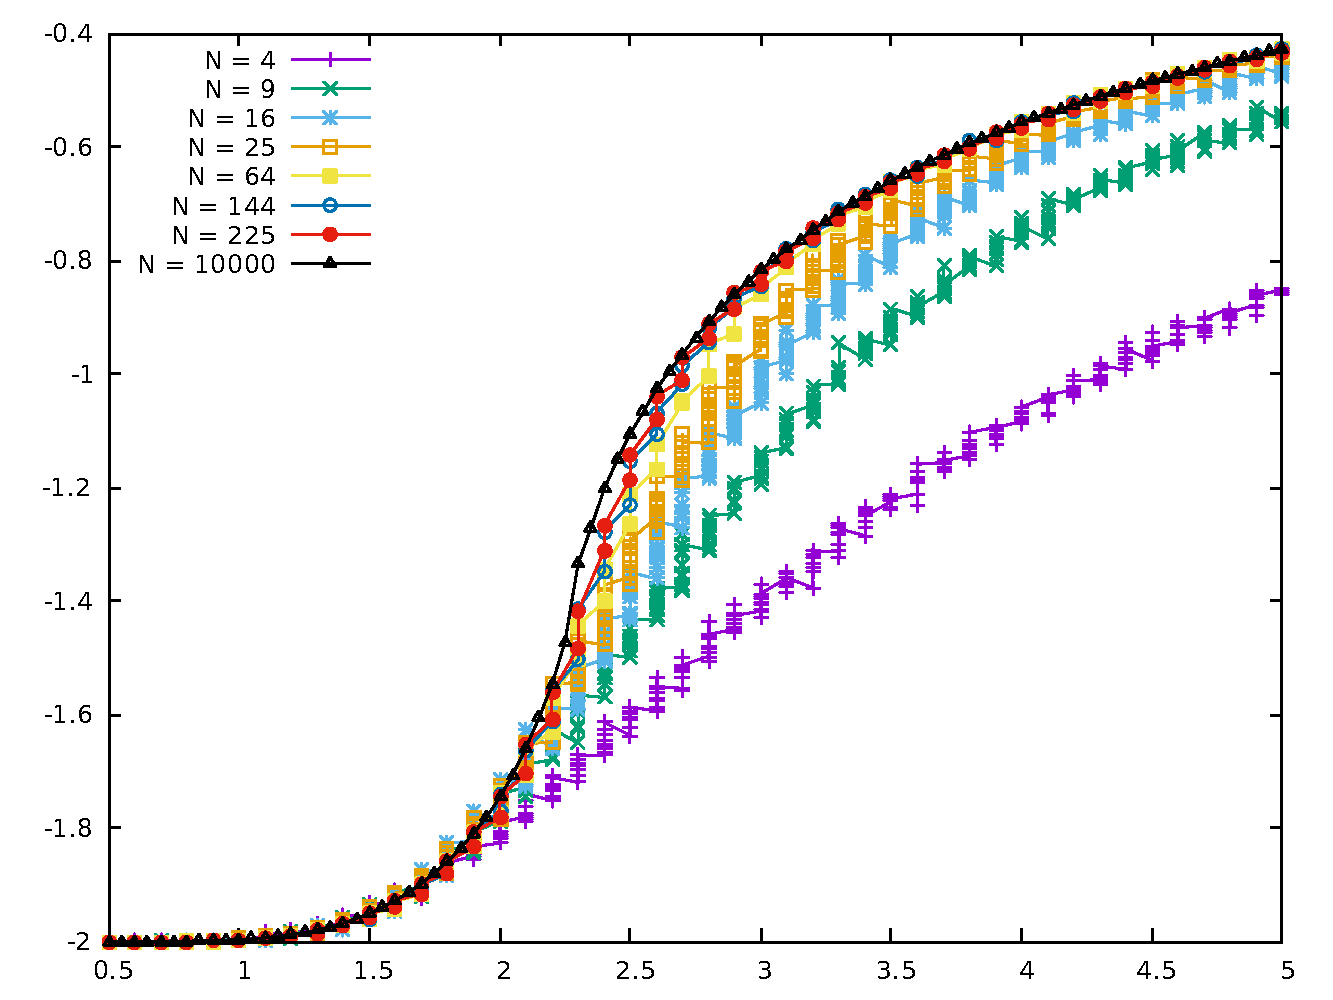
\includegraphics[scale=.35]{Energy.pdf}
	\caption{Energia média por spins (eixo vertial) para valores de $N=2$ até $N = 1000$. Eixo horizontal representando a temperatura.}
	\label{fig:II.2}
\end{figure}

Note que os gráficos parecem se aproximar de um gráfico limite, que parece começar a revelar uma descontinuidade na região de temperatura entre $2$ e $2.5$\footnote{Para a simulação definimos $J = k = 1$, visto que, segundo a solução de Onsager, o que importa é a razão $J/K$ para a temperatura de transição de fase.}

É importante citar que o cálculo feito acima se deu inicializando os spins de maneira aleatória. Compararemos com os resultados de uma outra forma de inicialização, ainda nesta subseção. Calculando a magnetização absoluta média, encontramos um resultado que parece colaborar para a ideia de surgir uma descontinuidade (Figura \ref{fig:II.3}).

\begin{figure}[h]
	\center
	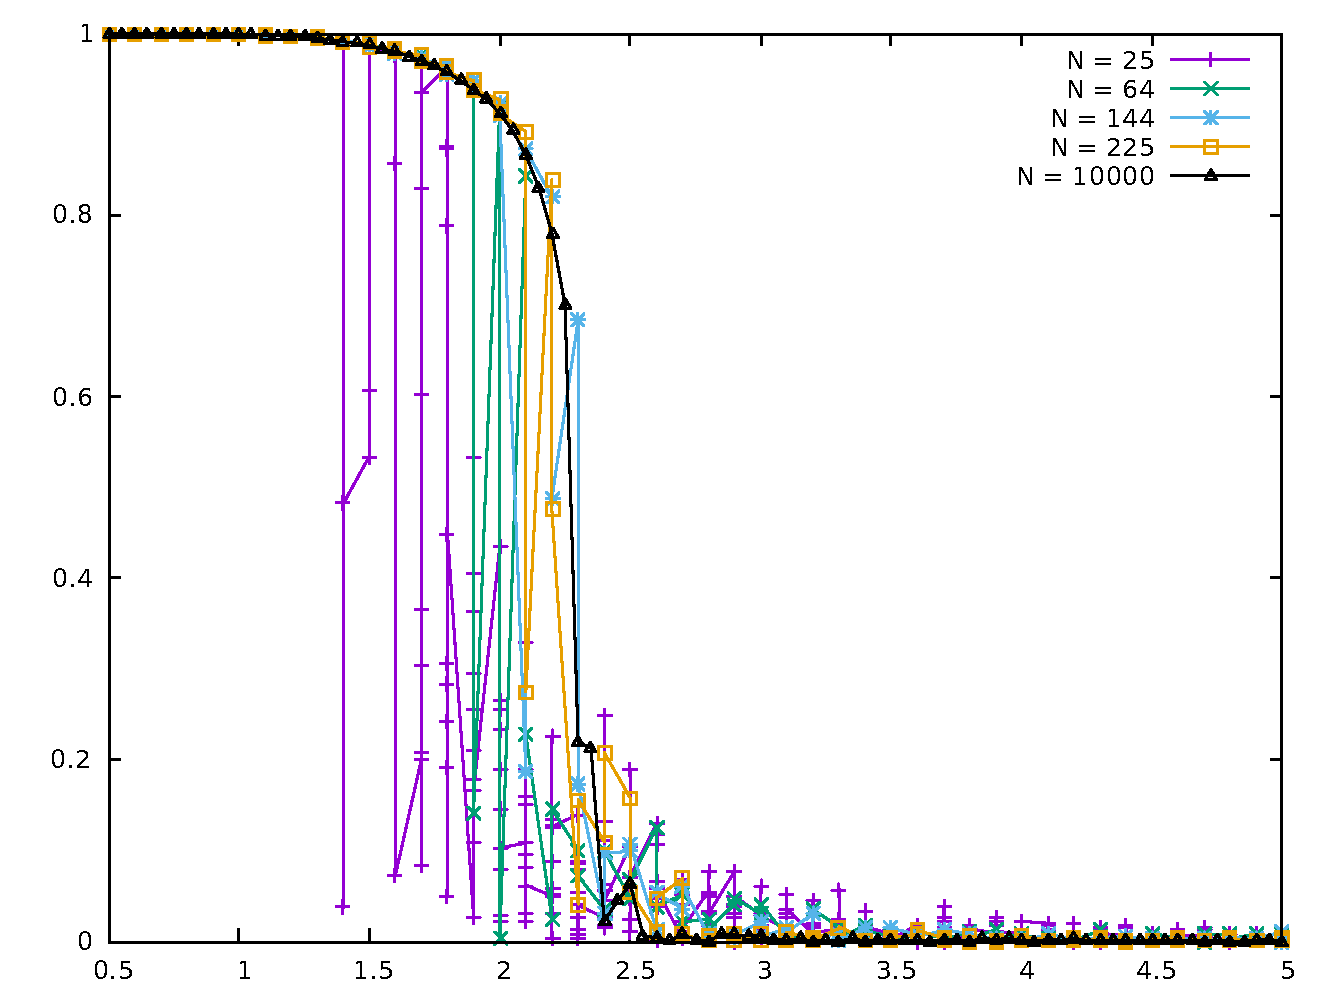
\includegraphics[scale=.35]{Magnetization.pdf}
	\caption{Magnetização absoluta média (eixo vertical) em função da temperatura (eixo horintal) variando-se as quantidades de spins de 25 até 1000.}
	\label{fig:II.3}
\end{figure}

Podemos notar que o resultado obtido para 10000 spins se aproxima muito da solução exata do modelo de Ising \cite{Baxter, Huang}. De fato, o gráfico esperado para a magnetização é como a Figura \ref{fig:II.4}.  



Com isso e com uma análise um pouco mais criteriosa do programa, podemos ter certeza que a implementação está correta e que nos dará os resultados esperados. Podemos partir para a introdução da anisotropia e calcular os observáveis quânticos.



\subsection{Observáveis Quânticos - Modelo Clássico Anisotrópico}
\label{subsec:ObservaveisQuanticosModeloAnisotropico}

A adaptação do programa para o modelo anisotrópico é feita de forma muito simples. Introduz-se um novo termo de acoplamento e adaptamos as expressões para os observáveis. A questão que surge é: quais valores adotar para os acoplamentos $J_x$ e $J_y$ nas direções verticais e horizontais, respectivamente? 

Esse problema pode ser resolvido utilizando-se algumas relações de simetria para o modelo. Pouco antes da solução de Onsager, na década de 40, ocorreu o descobrimento da \textit{dualidade de Kramers-Wannier}, uma relação de simetria que permitiu obter-se o diagrama de fase teórico para o modelo \cite{Kramers-1941I, Kramers-1941II}. 

O resultado do diagrama de fase devida a auto-dualidade do modelo pode ser estendida para o modelo quântico \cite{KogutMain}. Relacionando as variáveis clássicas e quânticas, podemos determinar a relação do acoplamento. 

Por questão de simplicidade, visto que os resultado para o modelo são apenas qualitativos; não utilizamos unidades reais para o calculo de algo, adotou-se $J_x = 0.03$ e $J_y = 0.97$. 



A simulação para os observáveis $\sz_i$ e $\sx_i$ estão mostradas nas Figuras \ref{fig:II.5} e \ref{fig:II.6}. 


Dos perfis observados para as funções de correlação, poderíamos ter a ideia de que uma descontinuidade nos observáveis envolvidos na desiguraldade de Bell via (\ref{eq:II.12}) se mostraria presente. Este é um resultado interessante. Havendo regiões onde a desigualdade é respeitada ou não nos levaria a encarar o diagrama de fases da rede como um diagrama de comportamento mais clássico e uma região de comportamento fortemente não-clássico. 

O comportamento presente na correlação para $\sx$ nos diz que a soma em (\ref{eq:II.12}) terá o mesmo perfil, visto que a descontinuidade na função se faz mais aparente do que a descontinuidade em sua derivda, para a soma dos observáveis da desigualdade de Bell. 

\begin{figure}[h]
	\center
	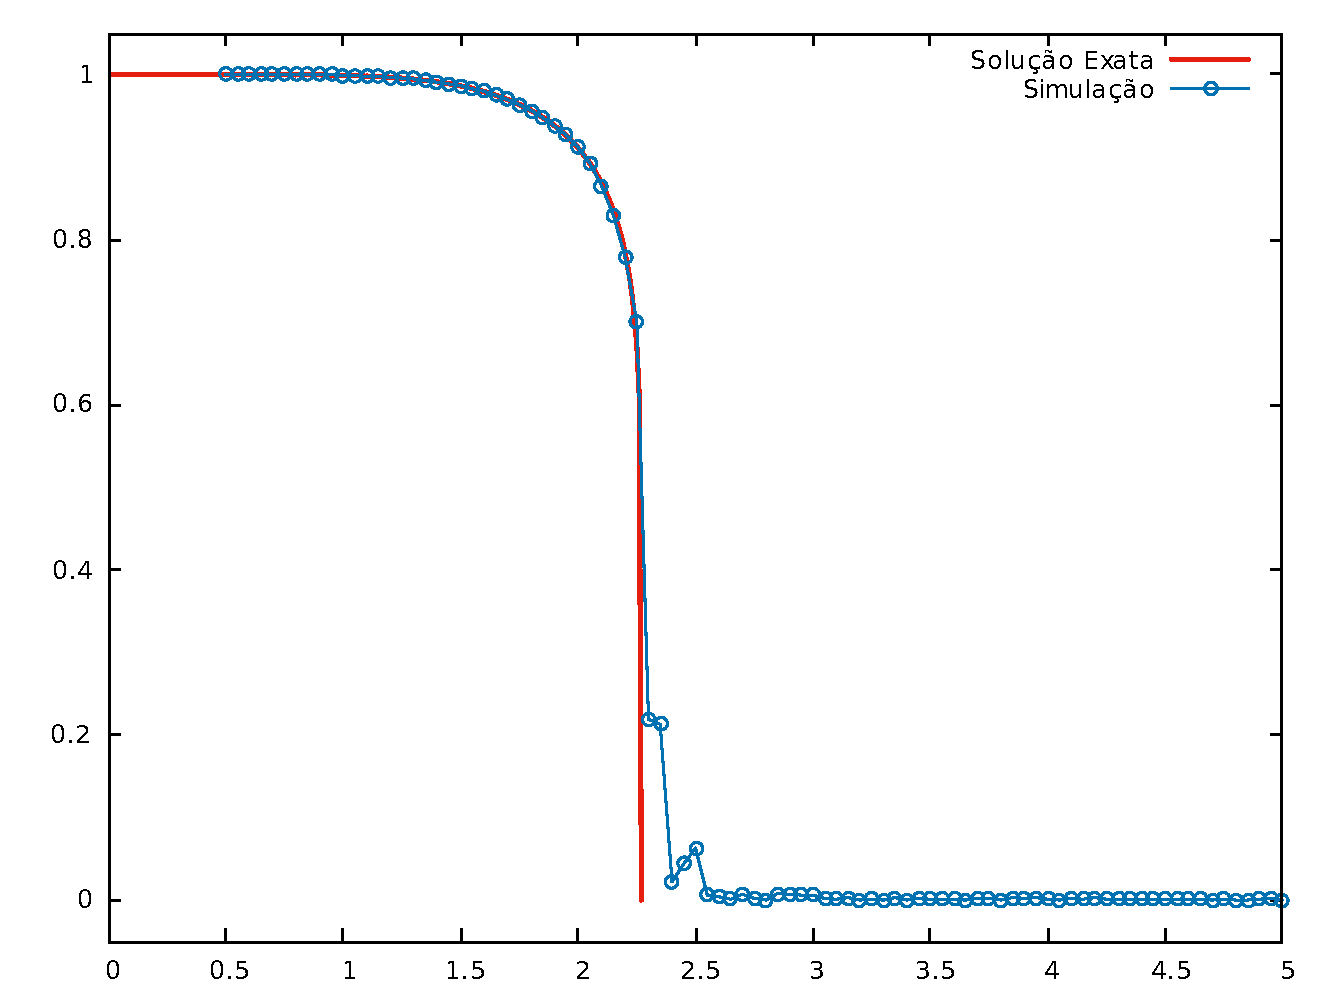
\includegraphics[scale=.3]{ExactMagnet.pdf}
	\caption{Comparação entre a simulação computacional (azul) e a solução exata de Onsager (vermelho)}
	\label{fig:II.4}
\end{figure}

\begin{figure}[h]
	\center
	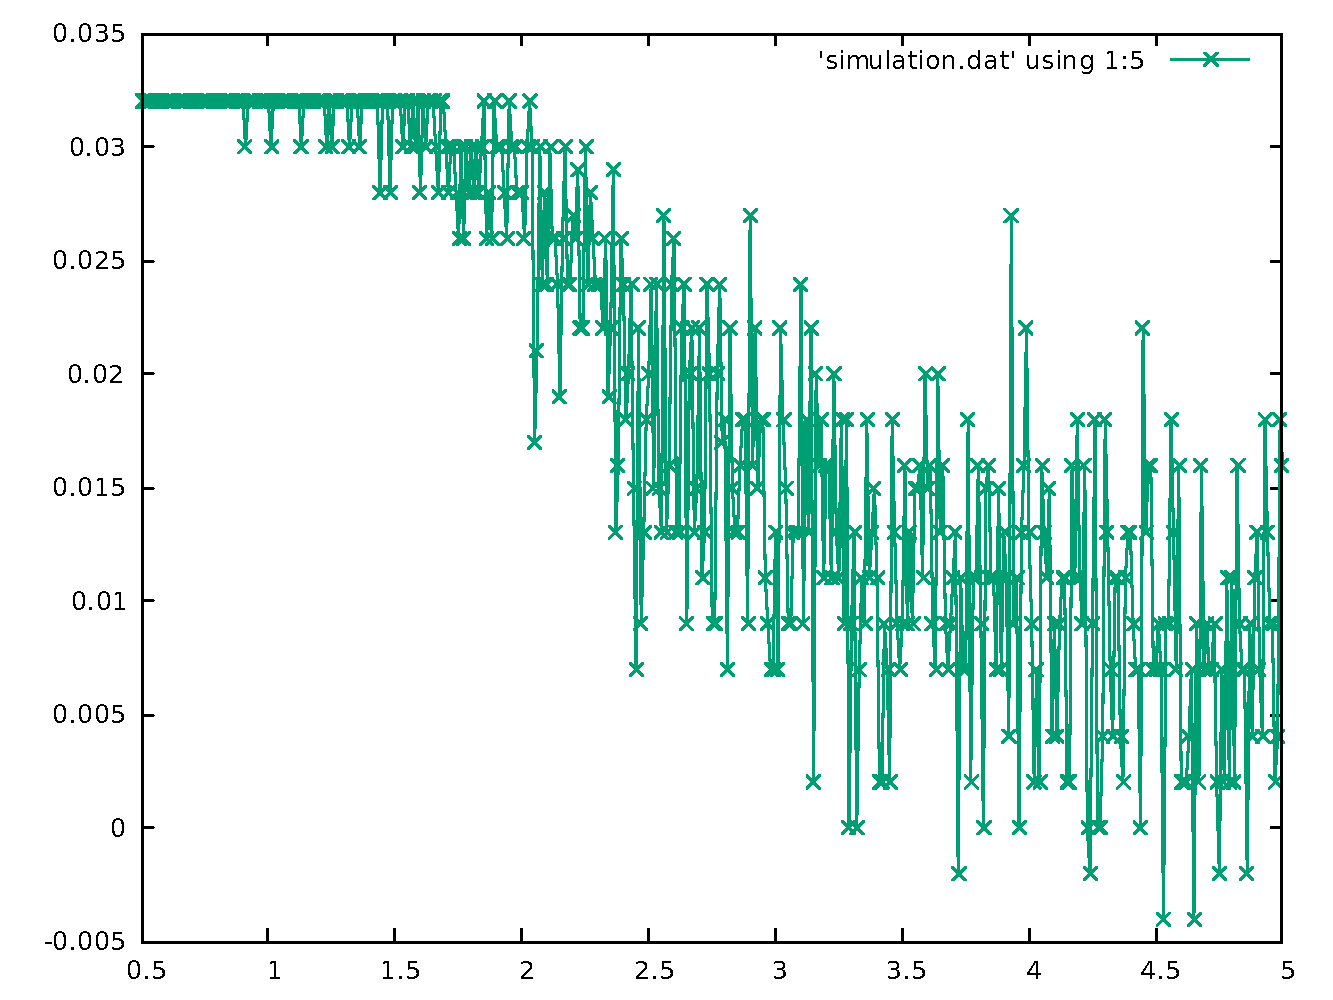
\includegraphics[scale=.3]{CorrSz.pdf}
	\caption{Função de correlação $\ev{\sz_i \sz_j} - \ev{\sz_i} \ev{\sz_j}$ (vertical) em função da temperatura (horizontal).}
	\label{fig:II.6}
\end{figure}


\begin{figure}[h]
	\center
	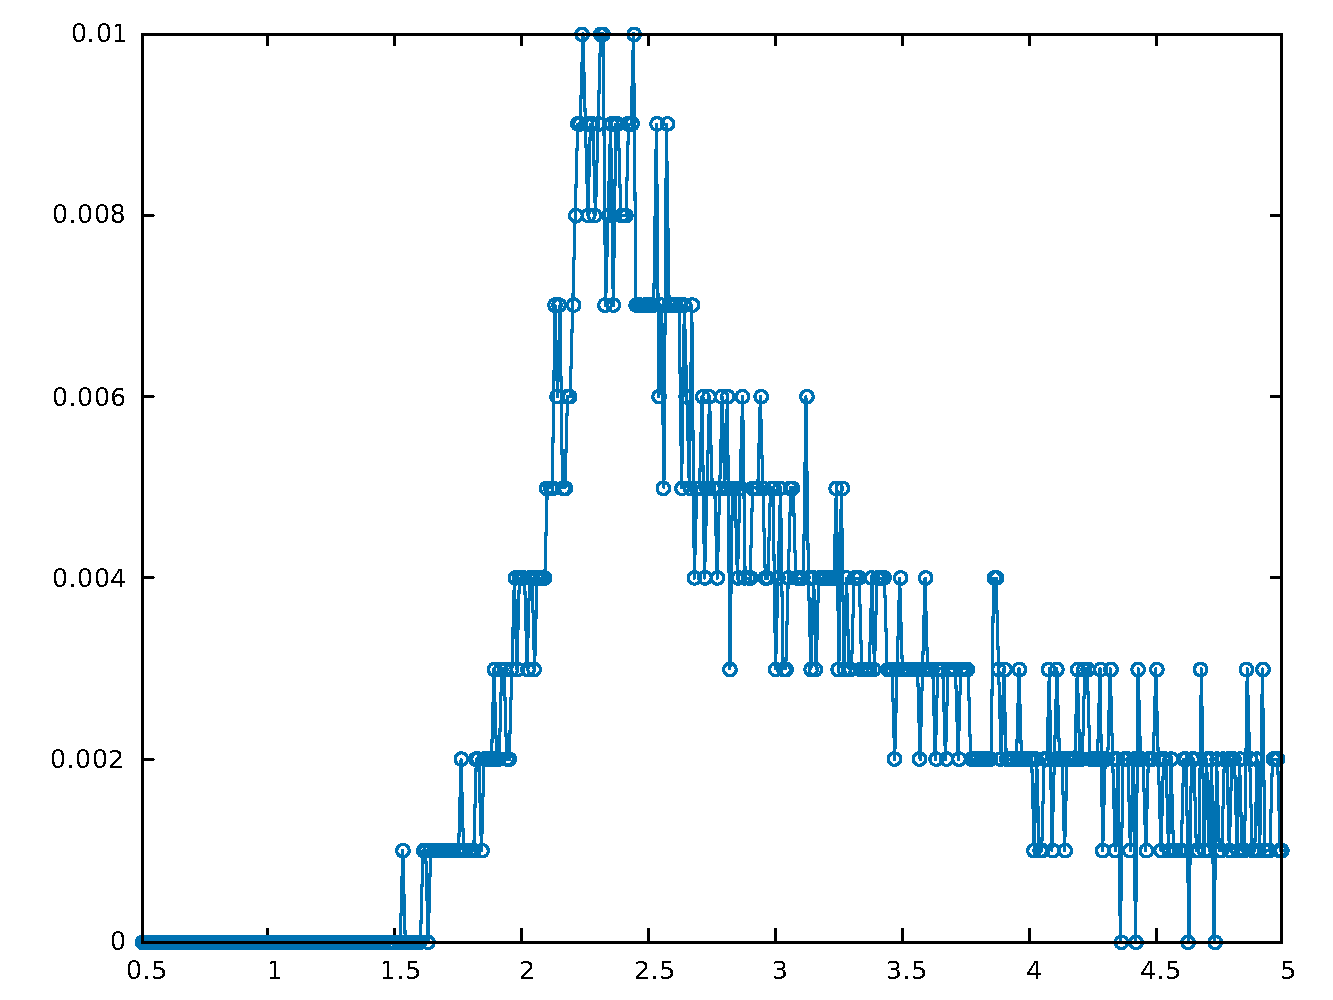
\includegraphics[scale=.3]{CorrSx.pdf}
	\caption{Função de correlação $\ev{\sx_i \sx_j} - \ev{\sx_i} \ev{\sx_j}$ (vertical) em função da temperatura (horizontal).}
	\label{fig:II.6}
\end{figure}



A Figura \ref{fig:II.7} ilustra o cálculo da soma em (\ref{eq:II.12}), variândo-se a temperatura. O resultado é o esperado. Vemos que sugere uma descontinuidade na região de transição de fase. A forma da descontinuidade é tal que, na transição, a desigualdade de Bell é violada. Isso representa que a transição de fase é o momento onde o sistema quântico se torna mais fortemente emaranhado. 

\begin{figure}[h]
	\center
	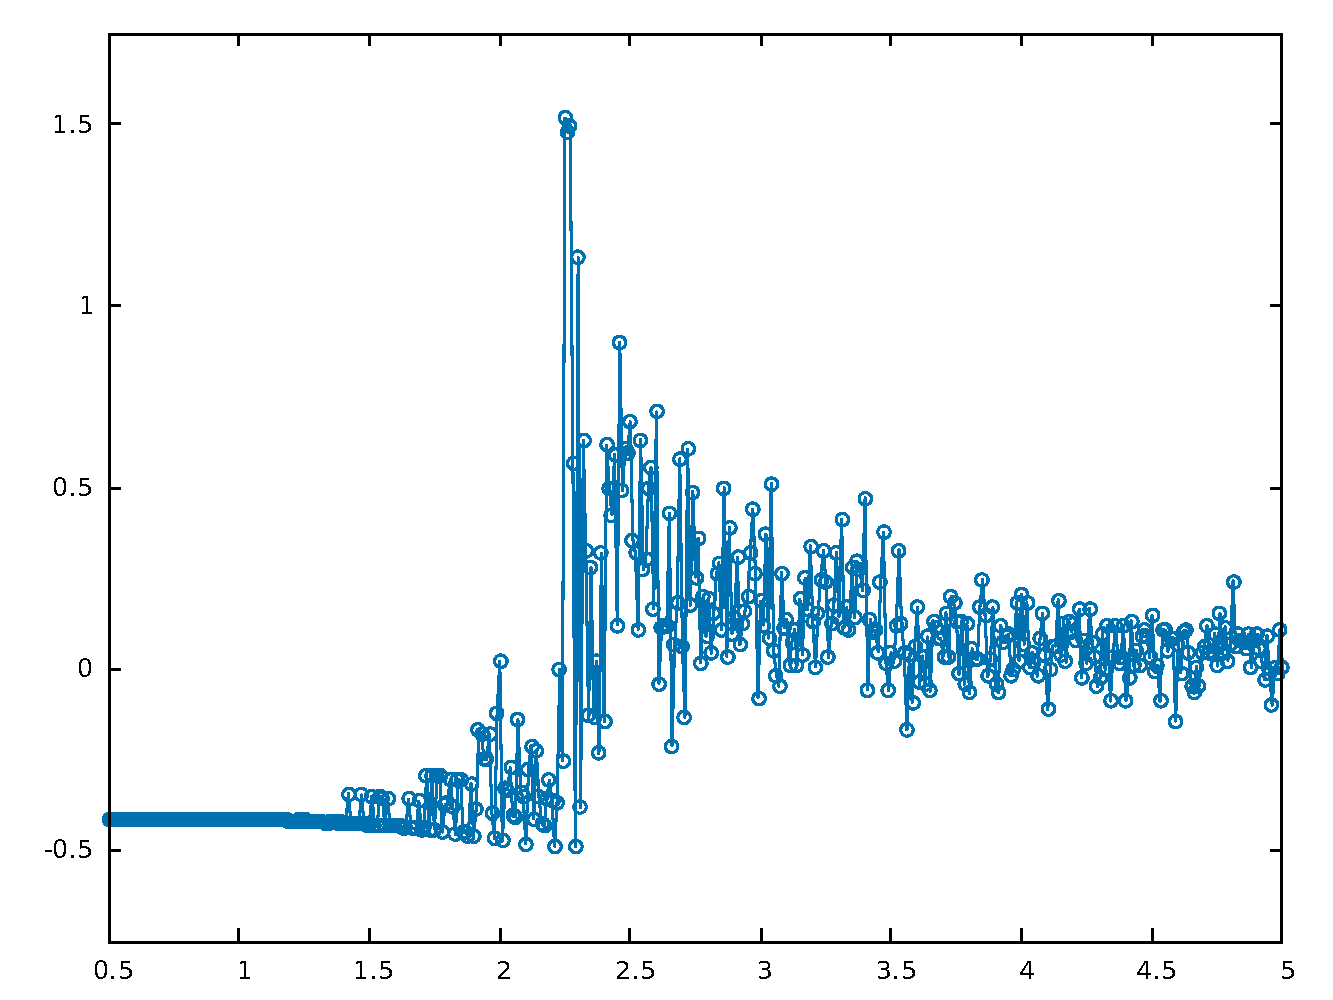
\includegraphics[scale=.3]{IsotropicMBell.pdf}
	\caption{Valores esperados da desigualdade de Bell  (\ref{eq:II.11})$-$(\ref{eq:II.12}) (eixo vertical) em função da temperatura (eixo horizontal).}
	\label{fig:II.7}
\end{figure}



\newpage

\section{Conclusão}
\label{sec:Conclusao}

Com os resultados apresentado, mostrou-se que medidas de emaranhamento podem ser calculadas fazendo uso de simulação computacional com o sistema clássico, por meio do mapeamento clássico-quântico. 

Através dos análogos clássicos para os observáveis quânticos, pôde-se estudar o comportamento de uma das desigualdades de Bell, em função da temperatura. O resultado obtido nos permitiu ver o regime de transição de fase como o regime pra o qual o sistema se encontra mais fortemente emaranhado, de tal forma que a localidade da medida é quebrada, com isso, o flip de um spin em uma posição da rede causa uma excitação que se propaga sem perda por distâncias infinitas, representando a divergência do comprimento de correlação da rede durante a transição, dado que a desigualdade de Bell passa a ser violada na temperatura de transição de fase.
Ao se afastar da transição, a desigualdade volta a ser respeitada.

Podemos entender este resultado como se a transição de fase no modelo quântico fosse uma transição do tipo localidade$-$não localidade. 

Os cálculos envolvidos foram da ordem de cinco minutos para uma rede $50 \times 50$, com 3000 iterações para o laço de Monte Carlo e o tamanho da rede para o laço do algoritmo de Metropolis. O tempo de processamento é razoávelmente baixo, visto que o problema é do tipo NP-complexo. Retomando a discução acerca da simulação direta do modelo quântico, é fácil perceber que a aplicação de diversas matrizes de ordem $50 \times 50$ em vetores de estado com $50$ componentes é um trabalho muito custoso. Assim, podemos concluir que a eficiência obtida por meio da técnica utilizada é alta, nos fornecendo bons resultados como visto em \ref{subsec:ObservaveisClassicosParaOModeloIsotropico} e \ref{subsec:ObservaveisQuanticosModeloAnisotropico}. 



\bibliographystyle{abbrv}
\addcontentsline{toc}{section}{Referências}
\bibliography{ref.bib}
\label{Referencias}


\end{document}